% UC-Bench portfolio report. Upload this file as main.tex to Overleaf.
% Compiler: pdfLaTeX. No shell escape, external images, or bibliography files.
% Evidence cutoff: 14 September 2026. Researcher-facing: contains case answers.
\documentclass[11pt,a4paper]{article}
\usepackage[T1]{fontenc}
\usepackage[utf8]{inputenc}
\usepackage{lmodern}
\usepackage[margin=22mm]{geometry}
\usepackage{microtype}
\usepackage{amsmath,amssymb}
\usepackage{graphicx}
\usepackage[table]{xcolor}
\usepackage{booktabs,longtable,tabularx,array}
\usepackage{enumitem}
\usepackage{float}
\usepackage{tikz}
\usetikzlibrary{arrows.meta,positioning,shapes.geometric,fit,calc}
\usepackage{pgfplots}
\pgfplotsset{compat=1.18}
\usepackage{xurl}
\usepackage{hyperref}
\usepackage{fancyhdr}
\usepackage{listings}
\definecolor{Ink}{HTML}{19334B}
\definecolor{Teal}{HTML}{087F8C}
\definecolor{Pale}{HTML}{EAF4F5}
\definecolor{Amber}{HTML}{9A6100}
\definecolor{Red}{HTML}{A83232}
\definecolor{Muted}{HTML}{52616B}
\hypersetup{colorlinks=true,linkcolor=Teal,urlcolor=Teal,citecolor=Teal,
  pdftitle={UC-Bench: Case 1 and Case 2 Pilot Evidence; Case 3 and Case 4 Development},
  pdfauthor={UC-Bench}}
\pagestyle{fancy}\fancyhf{}
\fancyhead[L]{\small\textcolor{Ink}{UC-Bench / technical report}}
\fancyhead[R]{\small 14 September 2026}
\fancyfoot[L]{\scriptsize Researcher-facing: contains evaluation answers}
\fancyfoot[R]{\thepage}
\setlength{\headheight}{15pt}
\setlength{\parindent}{0pt}
\setlength{\parskip}{6pt}
\setlength{\emergencystretch}{2em}
\renewcommand{\arraystretch}{1.18}
\setlist[itemize]{nosep,leftmargin=*}
\setlist[enumerate]{nosep,leftmargin=*}
\newcolumntype{Y}{>{\raggedright\arraybackslash}X}
\newcommand{\pass}{\textcolor{Teal}{Pass}}
\newcommand{\fail}{\textcolor{Red}{Fail}}
\newcommand{\missing}{\textcolor{Muted}{Missing}}
\newcommand{\na}{\textcolor{Muted}{N/A}}
\newcommand{\filepath}[1]{\nolinkurl{#1}}
\newcommand{\note}[1]{\begin{quote}\small\color{Muted}#1\end{quote}}
\tikzset{
 block/.style={draw=Ink!65,fill=Pale,rounded corners=3pt,align=center,
   font=\small,text width=4.1cm,minimum height=10mm,inner sep=5pt},
 neutral/.style={block,fill=white},
 gate/.style={block,fill=orange!12,draw=Amber},
 result/.style={block,fill=Teal!12,draw=Teal},
 arr/.style={-{Latex[length=2.1mm]},thick,draw=Ink!80},
 edge/.style={font=\scriptsize,fill=white,inner sep=2pt,align=center}
}
\lstset{basicstyle=\ttfamily\footnotesize,breaklines=true,columns=fullflexible,
 frame=single,rulecolor=\color{Ink!20},backgroundcolor=\color{black!2},
 keepspaces=true,showstringspaces=false}

\begin{document}
\begin{titlepage}
\vspace*{12mm}
{\Large\color{Teal}UC-Bench\par}
\vspace{8mm}
{\Huge\bfseries\color{Ink}Auditing the biomedical\newline evidence chain\par}
\vspace{8mm}
{\Large Case 1 and Case 2 pilot evidence\par}
{\Large Case 3 and Case 4 development portfolio\par}
\vspace{12mm}
\begin{tabularx}{\textwidth}{@{}lY@{}}
\toprule
Report date & 14 September 2026 \\
Scope & One locked anti-TNF predictor-diligence environment; four case packets and five controlled conditions. \\
Agent's job & Decide what the evidence supports, contain invalid claims, and select useful next evidence. Training a replacement predictor is not required. \\
Evidence level & Small controlled internal pilot, locally validated controls, and explicitly labeled development replays. \\
Distribution & Researcher-facing document containing hidden outcomes and reference answers. Keep outside all agent-visible workspaces. \\
\bottomrule
\end{tabularx}
\vfill
\textbf{Reading the results.} A mission pass means the agent completed the required investigation with supported decisions. Partial scientific quality measures verifiable work. Completion reliability measures submission, not scientific correctness. These quantities answer different questions.
\vspace{6mm}
\textcolor{Muted}{This document describes the inspected artifacts. Case 2's packaging manifest was still \texttt{candidate\_unfrozen} at the evidence cutoff; the report does not certify a later freeze.}
\end{titlepage}
\tableofcontents
\clearpage

\section{Executive assessment and release status}

Case 1 is an accepted final RC6 pilot. Two of four provider-eligible attempts passed the full mission; one completed with substantial scientific failures and one did not submit. Case 2 has a completed four-trajectory evidence set and accepted verifier replays after two general scoring corrections. All four missions failed, while independent scientific work earned substantial partial credit in three attempts. These are observations of different workflow outcomes, not stable rankings of models.

Case 3 has a locally validated development implementation with two controlled outcomes and six successful reference workflows. It has no model calibration under that candidate. Case 4 retains its historical packet and reference values; its current release audit and implementation remain future work.\cite{c1,c2optional,c3,c4status}

\begin{table}[H]\small
\caption{Release and evidence status at the report cutoff.}
\begin{tabularx}{\textwidth}{@{}lYY@{}}\toprule
Case & What exists & What can be claimed \\\midrule
1: sufficient bounded evidence & Accepted, frozen \texttt{case1-pilot-v1-rc6}; mixed RC5/RC6 trajectory provenance under RC6 grading & Demonstrated tractability, one scientific failure, one completion failure; one provider exclusion. \\
2: dependence and site effects & Locally validated repaired verifier; reproducible MMMVP package candidate; four replay-parity checks pass & Supported descriptive trajectory analysis. Final package manifest remains unfrozen. \\
3: provenance and re-execution & Unfrozen development candidate; collapse/remains outcomes; 102 focused tests & Local tractability and controls demonstrated; model performance unknown. \\
4: ranking versus useful probabilities & Historical packet, hidden returns, archived metrics and early implementation history & Task intent and assets documented; no current release-level validity claim. \\\bottomrule
\end{tabularx}
\end{table}

\textbf{What the product presently tests.} The environment tests structured scientific diligence: cohort definition, dependence handling, reproducible calculation, prospective commitment, evidence interpretation, and restricted development decisions. It provides schemas and supported numerical conventions. Its open-endedness lies in the evidence-supported choices within that interface; it does not measure unrestricted scientific method invention.

\textbf{What is not established.} No result identifies a training-data deficit, need for SFT or RL, optimal monetary value of information, clinical benefit, or a stable ordering of model families. Proposed remedies below are hypotheses unless an explicit control or intervention demonstrates them. No RL training run is claimed.

\section{Environment definition and shared workflow}
\subsection{Professional setting and intended use}

The agent acts as a computational biologist conducting predictor diligence with statistical and clinical input represented in the evidence room. The target population is adults with moderate-to-severe ulcerative colitis before first infliximab. Inputs are baseline measurements; the endpoint is clinical response near day 42, within days 35--49. Predictor outputs are prognostic probabilities for research-use triage. A predictor of response in treated patients does not, by itself, identify individual treatment benefit.\cite{runbook,packet4}

The controlled packets make the task executable without requiring the agent to train a transcriptomic model. Locked predictions, cohort metadata, endpoint evidence, processing lineage and resource returns provide the raw material. They should not be described as an authentic GEO validation result. Authentic source-cohort work, where available historically, remains a separate evidence track.

\subsection{Observation, action and host state}

One episode can be represented as a partially observed decision process. The agent observes public files, accepted tool results and its own work. The host retains unrevealed labels, unpurchased returns, grading logic and the authoritative event journal. An accepted action updates the phase; ordinary reads, code execution and recoverable validation errors do not relax an accepted commitment.

\begin{figure}[H]\centering
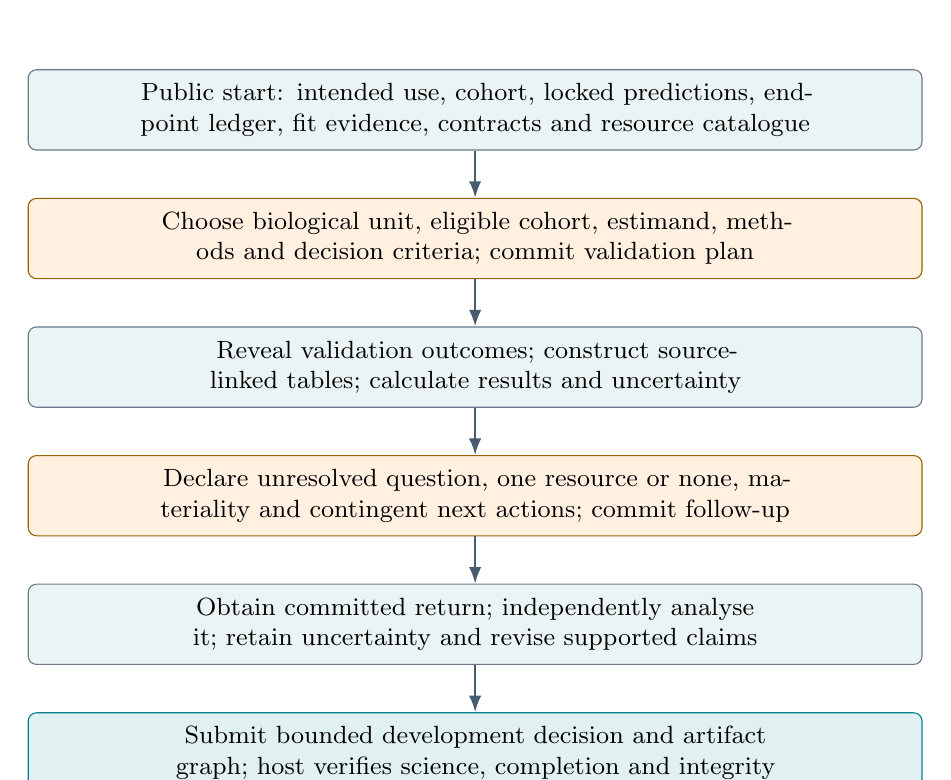
\begin{tikzpicture}[node distance=6mm]
\node[block,text width=11cm] (s0) {Public start: intended use, cohort, locked predictions, endpoint ledger, fit evidence, contracts and resource catalogue};
\node[gate,text width=11cm,below=of s0] (s1) {Choose biological unit, eligible cohort, estimand, methods and decision criteria; commit validation plan};
\node[block,text width=11cm,below=of s1] (s2) {Reveal validation outcomes; construct source-linked tables; calculate results and uncertainty};
\node[gate,text width=11cm,below=of s2] (s3) {Declare unresolved question, one resource or none, materiality and contingent next actions; commit follow-up};
\node[block,text width=11cm,below=of s3] (s4) {Obtain committed return; independently analyse it; retain uncertainty and revise supported claims};
\node[result,text width=11cm,below=of s4] (s5) {Submit bounded development decision and artifact graph; host verifies science, completion and integrity};
\foreach \a/\b in {s0/s1,s1/s2,s2/s3,s3/s4,s4/s5} \draw[arr] (\a)--(\b);
\end{tikzpicture}
\caption{Shared lifecycle. Orange nodes mark commitments before new evidence. A ``none'' purchase is an explicit no-new-evidence action, not an implicit bypass of the lifecycle.}
\end{figure}

\begin{table}[H]\small
\caption{Tools and boundaries. Exact field contracts remain in each case's public schema.}
\begin{tabularx}{\textwidth}{@{}lYY@{}}\toprule
Capability & Agent action & Host consequence \\\midrule
Inspect/read & List evidence; read public or revealed files & Observation only; no scientific score feedback. \\
Write/run code & Save scripts, tables and result files under \texttt{work/} & Derived work is retained; supplied evidence is protected. \\
\texttt{commit\_validation\_plan} & Submit cohort, methods, criteria and input references & Accept and hash a valid plan; return recoverable structural errors otherwise. \\
\texttt{reveal\_validation} & Request labels after commitment & Make sealed outcomes available and record ordering. \\
\texttt{commit\_followup\_plan} & State the question, resource, contingencies and evidence & Fix the prospective interpretation of the purchase. \\
\texttt{purchase\_resource} & Request the committed resource or none & Charge simulated units and expose only its return. \\
\texttt{submit} & Register final evidence and development decision & Accept terminal submission if the disclosed interface is valid; grade supported science independently. \\\bottomrule
\end{tabularx}
\end{table}

Model credentials, hidden evidence and host journals remain outside the Docker workspace. Agent internet access is disabled. Host persistence retains messages, returned reasoning state when supplied, tool calls/results, identities, usage and cost. Provider errors are handled separately from agent errors. These are tested engineering boundaries, not a proof that public biomedical literature is absent from model pretraining.

\subsection{Ten professional milestones}

The milestones below describe the full investigation, not ten independent tasks. Cases 1--2 use three substantive submission records and saved artifacts across five accepted lifecycle actions. Their scoring properties do not map one-to-one to milestones.

\begin{longtable}{@{}p{.06\textwidth}p{.24\textwidth}p{.32\textwidth}p{.29\textwidth}@{}}
\caption{Milestones, professional owners and consequential artifacts.}\label{tab:milestones}\\
\toprule M & Work / typical owner & Inspected or produced artifact & Consequence and accepted flexibility \\\midrule\endfirsthead
\toprule M & Work / typical owner & Inspected or produced artifact & Consequence and accepted flexibility \\\midrule\endhead
1 & Intended use / clinical and development lead & Population, input time, endpoint, allowed-use contract & Prevents a ranking result becoming a treatment-effect or clinical-use claim. A bounded stage decision is valid. \\
2 & Integrity and provenance / curator & Source files, manifests, hashes and sponsor assertions & Establishes which evidence can be trusted; missing history can remain unresolved. \\
3 & Patient and visit identity / curator and statistician & Cohort map, source memberships, exclusions and repeated records & Prevents pseudo-replication. Supported aggregation or clustered-row workflows may differ. \\
4 & Endpoint construction / clinical adjudicator & Endpoint-source ledger, date window and prospective ambiguity policy & Prevents mismatched or outcome-driven labels. Documented exclusions or a supported source hierarchy may be valid. \\
5 & Assay/preprocessing audit / platform specialist & Fit membership, preprocessing code/configuration, logs & Prevents unsupported independence or clean-execution claims. A provenance-limited conclusion is acceptable. \\
6 & Baseline reproduction / computational biologist & Source-linked analysis table and original metric outputs & Distinguishes a reported score from a reproducible calculation. Original performance can be calculated but judged ineligible. \\
7 & Validation commitment / statistician & Hashed plan, estimand, uncertainty, bins, threshold and criteria & Prevents selection after outcome reveal. Accepted commitments are immutable. \\
8 & Validation / statistician & AUC, interval, probability error, calibration, utility and site audit & Separates point accuracy, precision and context validity. Optional sensitivity work remains local. \\
9 & Follow-up / experimental-design lead & Question, chosen resource, contingencies, return and calculations & Purchase must inform the stated question. No purchase is valid when evidence already resolves it. \\
10 & Diligence decision / cross-functional lead & Decision tuple, claims, unresolved gates, next evidence and beliefs & Prevents unsupported advancement or unnecessary abandonment. Hold, scoped progression and stop require evidence. \\\bottomrule
\end{longtable}

\subsection{Evidence dependency graph}

\begin{figure}[H]\centering
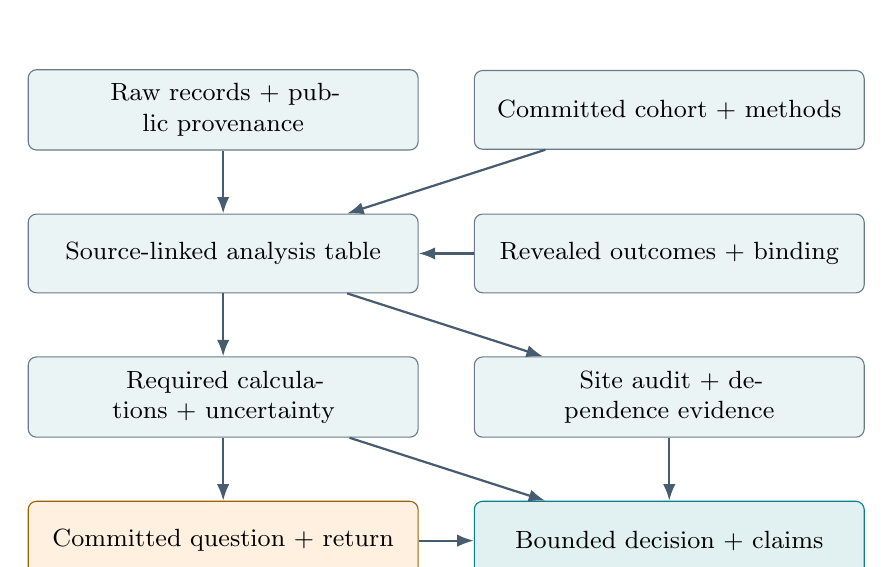
\begin{tikzpicture}[node distance=8mm and 7mm]
\node[block,text width=4.6cm] (raw) {Raw records + public provenance};
\node[block,text width=4.6cm,right=of raw] (plan) {Committed cohort + methods};
\node[block,text width=4.6cm,below=of raw] (table) {Source-linked analysis table};
\node[block,text width=4.6cm,right=of table] (out) {Revealed outcomes + binding};
\node[block,text width=4.6cm,below=of table] (calc) {Required calculations + uncertainty};
\node[block,text width=4.6cm,right=of calc] (site) {Site audit + dependence evidence};
\node[gate,text width=4.6cm,below=of calc] (purchase) {Committed question + return};
\node[result,text width=4.6cm,right=of purchase] (decision) {Bounded decision + claims};
\draw[arr] (raw)--(table);\draw[arr] (plan)--(table);
\draw[arr] (out)--(table);\draw[arr] (table)--(calc);\draw[arr] (table)--(site);
\draw[arr] (calc)--(purchase);\draw[arr] (calc)--(decision);\draw[arr] (site)--(decision);
\draw[arr] (purchase)--(decision);
\end{tikzpicture}
\caption{Conceptual dependency graph. Release-specific dependency tables are the authority for scoring. A broken downstream claim does not erase an independently verified upstream number.}
\end{figure}

\subsection{Follow-up resources}

The shared catalogue permits at most one purchase within three simulated units. Delay is a scenario attribute; it is not provider runtime or API spend. Titles describe what evidence can be obtained, not which purchase is always correct.

\begin{table}[H]\small
\begin{tabularx}{\textwidth}{@{}lYrrY@{}}\toprule
ID & Resource & Units & Days & Decision question it can address \\\midrule
X17 & Source-record reconciliation & 1 & 4 & Patient/visit identity; cannot supply new outcomes. \\
X24 & Endpoint evidence & 2 & 9 & Endpoint adjudication/provenance; cannot establish platform transport. \\
X31 & Pipeline execution & 1 & 5 & Processing lineage and executable return; cannot establish future clinical utility. \\
X46 & Matched external evidence & 3 & 21 & Transport in a matched setting, subject to actual predictor identity and scope. \\
X58 & Larger sample & 3 & 45 & Precision and sample coverage; more observations do not remove systematic bias. \\
X63 & Expert review & 1 & 3 & Methods interpretation; advice alone is not new empirical validation. \\
none & Purchase nothing & 0 & 0 & Appropriate when the bounded immediate question is resolved. \\\bottomrule
\end{tabularx}
\caption{Existing public catalogue. Return content and relevance are case-specific.}
\end{table}

\section{Measurement and scoring}
\subsection{Scientific calculations}

For a committed biological-unit table with weights $w_i$, scores $p_i$ and labels $y_i\in\{0,1\}$, the main quantities are:
\begin{align}
\operatorname{AUC}&=\frac{\sum_{i:y_i=1}\sum_{j:y_j=0}w_iw_j
 [\mathbf{1}(p_i>p_j)+\tfrac12\mathbf{1}(p_i=p_j)]}
 {\left(\sum_{i:y_i=1}w_i\right)\left(\sum_{j:y_j=0}w_j\right)},\\
\operatorname{Brier}&=\frac{\sum_i w_i(p_i-y_i)^2}{\sum_i w_i},\\
\operatorname{ECE}_{B}&=\sum_{b=1}^{B}\frac{W_b}{W}
 \left|\overline{p}_b-\overline{y}_b\right|,\\
\operatorname{NB}(t)&=\frac{\operatorname{TP}_w(t)}{W}
 -\frac{\operatorname{FP}_w(t)}{W}\frac{t}{1-t}.
\end{align}
Bins, membership, weighting and threshold must follow the committed public convention. Empty ECE bins contribute zero. At $t=0.5$, net benefit reduces to $(\operatorname{TP}_w-\operatorname{FP}_w)/W$. A positive net benefit relative to treating none does not demonstrate benefit relative to every alternative or prove clinical impact.

Uncertainty must resample the supported biological unit or cluster, not independent biopsy rows. Replicates, interval level, seed and numerical convention are committed. The reported examples use different valid cohorts, aggregation rules and interval settings; identical AUC with different ECE or intervals can therefore be legitimate. Case 2 discloses 2--20 calibration bins and 100--2000 resampling replicates. Required discrimination uncertainty stays strict; invalid optional intervals remain diagnostic unless a disclosed causal rule makes them decision-critical.

\subsection{Mission, scientific quality and reliability}

Let $E$ indicate a provider-eligible episode, $C$ an accepted final submission, and $P_k$ the required property outcomes. The mission result is
\begin{equation}
 M=C\land\bigwedge_{k\in\mathcal A}P_k,\qquad
 R=100\mathbf{1}(C)\quad\text{for eligible attempts}.
\end{equation}
Provider/infrastructure exclusions are reported outside the scientific denominator. Direct partial quality uses supported property subchecks $q_k\in[0,1]$ and fixed weights:
\begin{equation}
 Q=100\frac{\sum_{k\in\mathcal A} w_k q_k}{\sum_{k\in\mathcal A}w_k}.
\end{equation}
This equation summarizes the implemented weighting, not an alternative grader. Property subchecks, causal consequences and applicability are defined by the release. In particular, $Q$ is not a cutoff for $M$.

\begin{table}[H]\small
\caption{Property weights. Case 2 removes belief from strict scoring and renormalizes the remaining 93 weight units.}
\begin{tabularx}{\textwidth}{@{}Yrr@{}}\toprule
Property & Case 1 / 100 & Case 2 / 93 \\\midrule
Prospective design and integrity & 15 & 15 \\
Saved artifact chain & 10 & 10 \\
Entity and dependence analysis & 15 & 15 \\
Discrimination and uncertainty & 10 & 10 \\
Probability and calibration & 10 & 10 \\
Threshold utility & 8 & 8 \\
Context robustness & 8 & 8 \\
Decision-relevant follow-up & 10 & 10 \\
Belief revision & 7 & Diagnostic only \\
Bounded decision and claims & 7 & 7 \\\bottomrule
\end{tabularx}
\end{table}

Case 1's accepted report assigns no scientific score to its non-submitting Gemini attempt. Case 2 retains verifiable registered work for non-submitters. Case 1's mean of 79 is therefore a mean over three scoreable submissions; it must not be pooled with Case 2 means over all eligible episodes.

\subsection{Exact rules and open choices}

Machine-readable enums, fields, artifact references and chronology are enforced. Professional prose is retained for audit but does not independently determine strict outcomes through phrase matching. This protects paraphrases while limiting what the scorer can infer about nuanced reasoning. Scientific alternatives are accepted only within the disclosed supported interface; an arbitrary statistically defensible method is not automatically executable by every released verifier.

\section{Case 1: sufficient evidence for a bounded next stage}
\subsection{Task card}

\textbf{Scientific question.} Does the locked predictor support research probability development in the stated cohort, despite limited data-room imperfections, and is another purchase needed for that immediate decision?

\textbf{Start state.} The underlying packet has 134 source records representing 124 people. It supplies predictions, patient-linkage and endpoint provenance, fit evidence, intended use and the resource catalogue. Outcomes are withheld until commitment. The final RC5/RC6 public trees contain 40 identical files. One unresolved included endpoint-provenance flag matters to a possible X24 purchase.\cite{c1}

\textbf{Required work.} Define the eligible cohort, handle repeated records, commit analysis settings, reproduce discrimination and its interval, probability accuracy, calibration, utility and site sensitivity, then choose a follow-up and a bounded claim. The plan can justify exclusion before reveal; two passing agents used 123 people.

\textbf{Consequential alternatives.} No purchase is supported when the immediate question is resolved and no included provenance flag remains. With all 124 people included, X24 can resolve an endpoint-provenance question even if no label flips. Other resources require a supported question and valid use of the returned evidence. An expensive reassurance purchase is not automatically useful.

\textbf{Success.} The numerical and provenance chain supports the declared next stage, with clinical decision support, treatment selection and unjustified transport claims prohibited. A clinical deployment recommendation does not follow from this case.

\begin{figure}[H]\centering
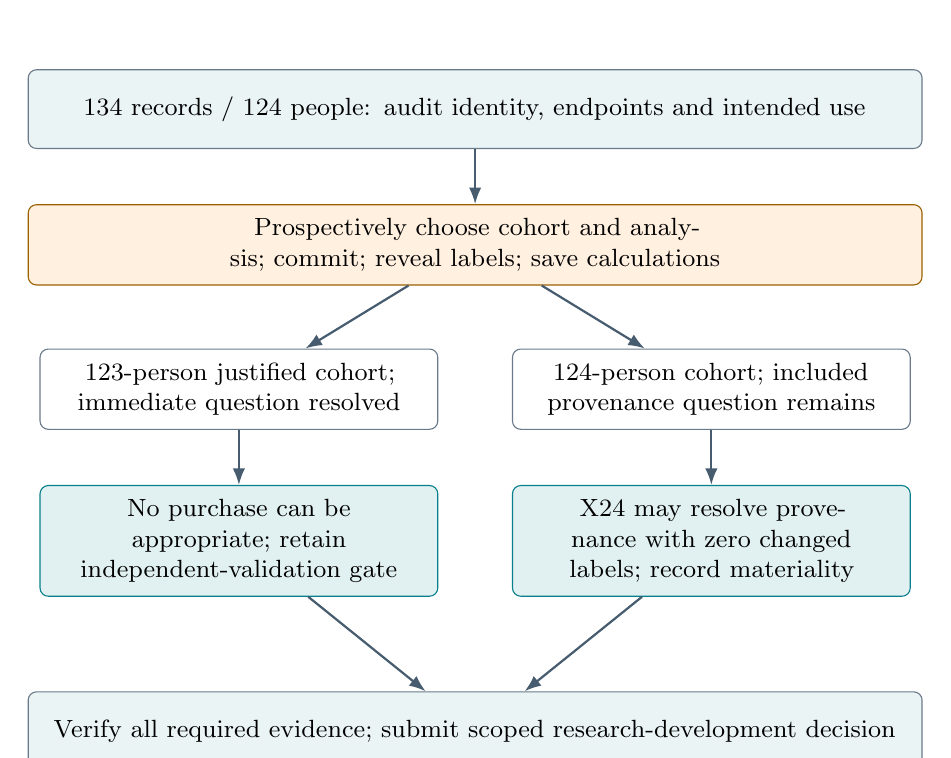
\begin{tikzpicture}[node distance=7mm and 8mm]
\node[block,text width=11cm] (a) {134 records / 124 people: audit identity, endpoints and intended use};
\node[gate,text width=11cm,below=of a] (b) {Prospectively choose cohort and analysis; commit; reveal labels; save calculations};
\node[neutral,text width=4.7cm,below=8mm of b.south,xshift=-3cm] (c) {123-person justified cohort; immediate question resolved};
\node[neutral,text width=4.7cm,below=8mm of b.south,xshift=3cm] (d) {124-person cohort; included provenance question remains};
\node[result,text width=4.7cm,below=of c] (e) {No purchase can be appropriate; retain independent-validation gate};
\node[result,text width=4.7cm,below=of d] (f) {X24 may resolve provenance with zero changed labels; record materiality};
\node[block,text width=11cm,anchor=north] (g) at ($(e.south)!0.5!(f.south)+(0,-1.2)$) {Verify all required evidence; submit scoped research-development decision};
\draw[arr] (a)--(b);\draw[arr] (b)--(c);\draw[arr] (b)--(d);
\draw[arr] (c)--(e);\draw[arr] (d)--(f);\draw[arr] (e)--(g);\draw[arr] (f)--(g);
\end{tikzpicture}
\caption{Case 1's demonstrated branches. They are evidence-dependent alternatives, not a universal instruction to exclude a patient or buy X24.}
\end{figure}

\subsection{Final RC6 pilot results}

\begin{table}[H]\small
\begin{tabularx}{\textwidth}{@{}Ylrrlr@{}}\toprule
Model & Mission & $Q$ & $R$ & Turns / requests$^*$ & USD \\\midrule
GPT-5 & Pass & 100 & 100 & 46 / 47 & 0.579765 \\
Sonnet 4 & Fail & 37 & 100 & 61 / 62 & 8.935311 \\
Gemini 3.1 Pro & Incomplete & N/A & 0 & 64 / 65 & 1.054765 \\
GPT-5.1 & Pass & 100 & 100 & 65 / 48 & 0.787011 \\
Opus 4.1 & Excluded & N/A & N/A & 47 / 48 attempts & 25.534605 \\\bottomrule
\end{tabularx}
\caption{Accepted RC6 report. GPT-5 and Sonnet are RC5 trajectories graded offline by RC6; Gemini and GPT-5.1 are fresh RC6 episodes. Opus is a preserved RC5 provider exclusion.}
\end{table}
\note{$^*$The accepted report calls these durable tool-turn counts. Raw RC6 run summaries instead store \texttt{turn\_count}=65 for Gemini and 47 for GPT-5.1. Both representations are preserved; physical request counts are the comparable transport measure. They must not be silently merged into a universal ``turn'' statistic.}

Mission success is $2/4=50\%$ among provider-eligible attempts; completion is $3/4=75\%$. The scoreable-submission mean is $(100+37+100)/3=79$. Among completed submissions, $2/3$ pass. One additional provider attempt is excluded. These tiny denominators do not support population estimates or a model-family ranking.

\begin{table}[H]\small
\caption{All ten Case 1 scientific properties for scoreable submissions.}
\begin{tabularx}{\textwidth}{@{}Yrrr@{}}\toprule
Property & GPT-5 & Sonnet 4 & GPT-5.1 \\\midrule
Prospective integrity & Pass & Pass & Pass \\
Artifact chain & Pass & Fail & Pass \\
Entity/dependence & Pass & Pass & Pass \\
Discrimination/uncertainty & Pass & Fail & Pass \\
Probability/calibration & Pass & Fail & Pass \\
Utility & Pass & Fail & Pass \\
Context robustness & Pass & Fail & Pass \\
Follow-up & Pass & Fail & Pass \\
Belief revision & Pass & Pass & Pass \\
Bounded claims & Pass & Fail & Pass \\\bottomrule
\end{tabularx}
\end{table}

\subsection{Numerical evidence and decisions}

\begin{table}[H]\small
\caption{Saved passing calculations. Minor rounding follows the preserved files.}
\begin{tabularx}{\textwidth}{@{}Yrr@{}}\toprule
Quantity & GPT-5 & GPT-5.1 \\\midrule
Included people & 123 & 123 \\
ROC AUC & 0.784881 & 0.784881 \\
Committed AUC interval & [0.719725, 0.849206] & [0.696986, 0.854762] \\
Interval level; replicates; seed & 90\%; 600; 20260911 & 95\%; 600; 41 \\
Brier score & 0.191344 & 0.191344 \\
Calibration error & 0.062100 & 0.095814 \\
Net benefit at 0.5 & 0.170732 & 0.170732 \\
Worst-site AUC & 0.694118 & 0.694118 \\
Site-weighted AUC & Not tabulated & 0.787427 \\
Log loss (extra diagnostic) & Not tabulated & 0.567076 \\
Purchase & none & none \\\bottomrule
\end{tabularx}
\end{table}

Calibration values need not coincide because calibration is tied to each committed calculation configuration. Interval levels and seeds also differ. Both workflows passed RC6 verification. GPT-5 retained its two beliefs at 0.60/0.40; GPT-5.1 retained 0.50/0.50. Their decisions allow scoped research development and leave external/clinical gates unresolved.

Sonnet included all 124 people and selected X24. It saved a valid primary table, but omitted calculation outputs from the artifact manifest and linked five primary calculations to a resource summary. It also used incorrect disclosed parameter keys for calibration and utility. Its declaration that resolving an included provenance question was immaterial was wrong even though zero labels changed. Its beliefs moved 0.60 to 0.85 and 0.40 to 0.15; the belief property passed, while the final claim remained unsupported by its artifact chain.

\subsection{Failure causality and engineering interpretation}

\begin{figure}[H]\centering
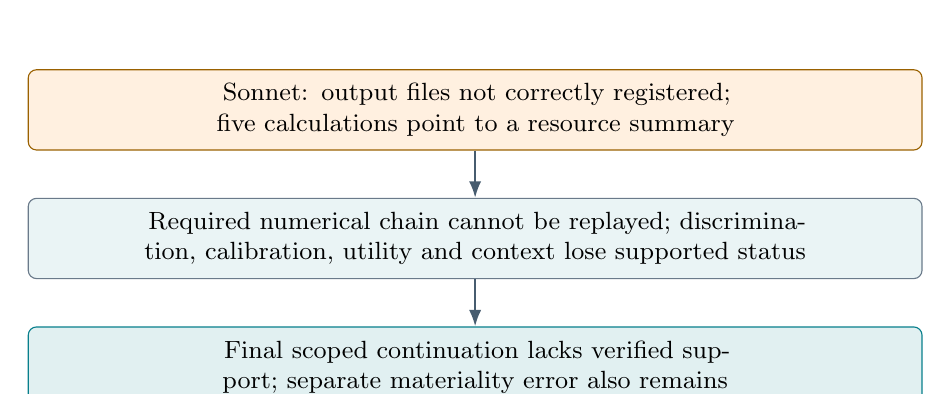
\begin{tikzpicture}[node distance=6mm]
\node[gate,text width=11cm] (a) {Sonnet: output files not correctly registered; five calculations point to a resource summary};
\node[block,text width=11cm,below=of a] (b) {Required numerical chain cannot be replayed; discrimination, calibration, utility and context lose supported status};
\node[result,text width=11cm,below=of b] (c) {Final scoped continuation lacks verified support; separate materiality error also remains};
\draw[arr] (a)--(b);\draw[arr] (b)--(c);
\end{tikzpicture}
\caption{First decision-critical failure and downstream consequences. Correcting every identified evaluator defect while retaining authored work leaves Sonnet at 37/fail. Repairing authored artifact links in a diagnostic counterfactual raises it to 70/fail; other errors remain. This is not a measured model intervention rescue.}
\end{figure}

Gemini reached the response boundary while debugging its own calculations, after committing a no-purchase plan. It did not submit. Opus's 48th request timed out after 47 exact model/provider identities; a missing response supplies no evidence of model substitution. RC6 correctly records a provider exclusion with no scientific or reliability score.

Two one-shot perfect completions give a case-level ceiling warning, not saturation. The one scoreable scientific failure begins at artifact binding, so its observed first-failure concentration is $1/1$; this is too small to characterize a general bottleneck. Completion friction warrants measurement even though two other agents finished. The task's professional requirement to preserve evidence links should not be confused with evidence that every amount of schema work is necessary.

\section{Case 2: dependence, context robustness and evidence use}
\subsection{Task card}

\textbf{Scientific question.} Does the apparent predictor performance survive reconstruction of biological units and examination of uneven site composition, and which next evidence can resolve the remaining development question?

\textbf{Start state.} The 25-file public environment contains 203 source records, locked predictions, identity/provenance information, endpoint evidence, processing files, a complete interface, and the resource catalogue. Provisional fingerprint groups are not automatically verified patient identities. Observed workflows retained 96 groups or prospectively excluded four groups to analyse 92. Outcomes remain hidden before commitment.

\textbf{Required calculations.} Reconstruct the committed source membership; calculate discrimination and required uncertainty, Brier score, calibration, threshold utility and site-specific/context results. Save source-record and entity counts separately. If new evidence is purchased, recompute and bind its results to the committed question and final action.

\textbf{Meaningful choices.} Supported aggregation versus clustered-row estimands; justified endpoint exclusions; whether identity or transport is the live question; X17, X46 or no purchase where supported; and a scoped continuation, pause or stop justified by the actual evidence. Neither a named defect nor a universal resource/action label is sufficient.

\textbf{Professional consequence.} Repeated biopsies can create false precision and an outcome-associated site mixture can inflate pooled ranking. Correctly reporting a pooled AUC does not establish robust use across sites.

\begin{figure}[H]\centering
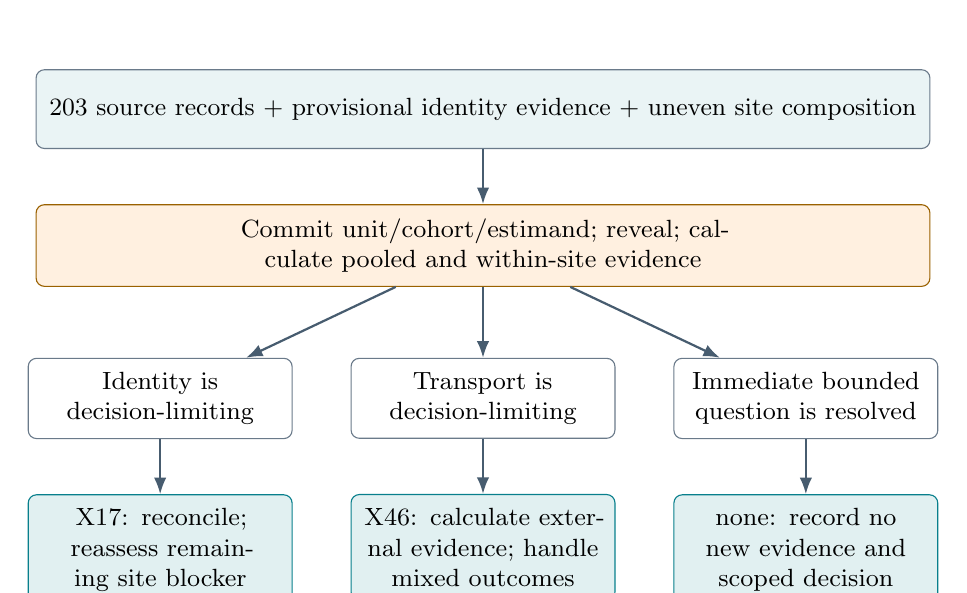
\begin{tikzpicture}[node distance=7mm and 6mm]
\node[block,text width=11cm] (a) {203 source records + provisional identity evidence + uneven site composition};
\node[gate,text width=11cm,below=of a] (b) {Commit unit/cohort/estimand; reveal; calculate pooled and within-site evidence};
\node[neutral,text width=3.0cm,below=9mm of b.south,xshift=-4.1cm] (c) {Identity is decision-limiting};
\node[neutral,text width=3.0cm,below=9mm of b] (d) {Transport is decision-limiting};
\node[neutral,text width=3.0cm,below=9mm of b.south,xshift=4.1cm] (e) {Immediate bounded question is resolved};
\node[result,text width=3.0cm,below=of c] (f) {X17: reconcile; reassess remaining site blocker};
\node[result,text width=3.0cm,below=of d] (g) {X46: calculate external evidence; handle mixed outcomes};
\node[result,text width=3.0cm,below=of e] (h) {none: record no new evidence and scoped decision};
\draw[arr] (a)--(b);\draw[arr] (b)--(c);\draw[arr] (b)--(d);\draw[arr] (b)--(e);
\draw[arr] (c)--(f);\draw[arr] (d)--(g);\draw[arr] (e)--(h);
\end{tikzpicture}
\caption{Case 2's question-dependent branch map. Actual valid paths depend on the committed cohort, public resource rules and calculated evidence. The X46 branch is the one observed in the three further-progressing trajectories.}
\end{figure}

\subsection{Four trajectories and score provenance}

The initial three-model run spent \$9.4419394. A later Sonnet canary spent \$8.803284 to check a general scorer correction on a fresh artifact chain. That canary is an extra attempt, not a fourth model in a balanced comparison. Accepted optionality replays and the package parity record agree.\cite{c2run,c2diag,c2canary,c2optional,c2package}

\begin{table}[H]\small
\begin{tabularx}{\textwidth}{@{}Yrrrrlr@{}}\toprule
Attempt & Raw $Q$ & Replay $Q$ & $M$ & $R$ & Turns / req. & USD \\\midrule
Gemini & 16.129032 & 16.129032 & 0 & 0 & 65 / 65 & 0.877291 \\
GPT-5.1 & 65.909091 & 65.909091 & 0 & 100 & 51 / 53 & 1.170929 \\
Sonnet, initial & 43.010753 & 61.290323 & 0 & 0 & 65 / 65 & 7.393719 \\
Sonnet, canary & 77.419355 & 77.419355 & 0 & 0 & 65 / 65 & 8.803284 \\\bottomrule
\end{tabularx}
\caption{Raw frozen outputs and accepted development-verifier replays, preserved side by side. No historical score is overwritten. $M=0$ denotes failed complete mission, including noncompletion.}
\end{table}

The initial balanced panel has $0/3$ missions and $1/3$ accepted submissions; its mean replay quality is 47.776149. Across all four attempts, missions remain $0/4$ and completion is $1/4$. The four-attempt mean of 55.186975 is only an attempt-weighted descriptive number: it overweights Sonnet and is not a cross-model aggregate. Higher partial quality does not convert a non-submission into a mission pass.

\begin{figure}[H]\centering
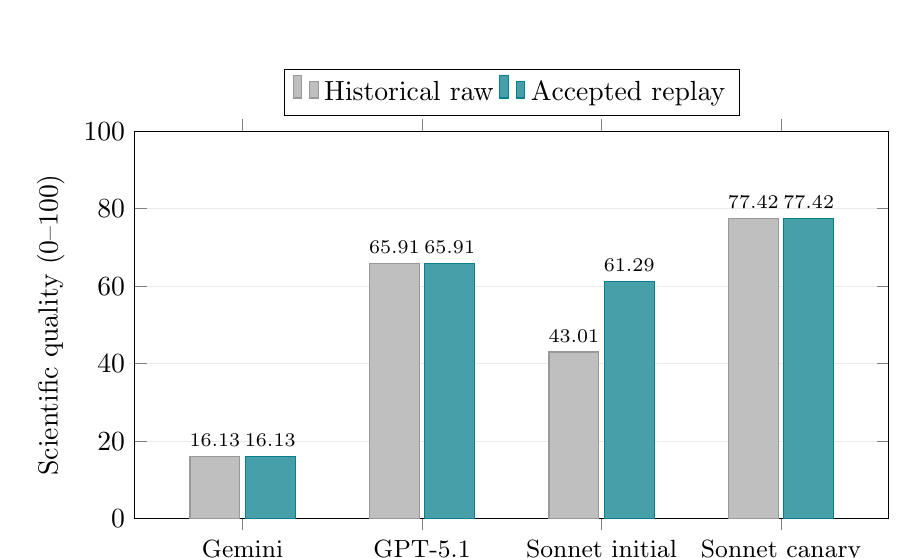
\begin{tikzpicture}
\begin{axis}[ybar,bar width=18pt,width=.92\textwidth,height=6.5cm,
 ymin=0,ymax=100,ylabel={Scientific quality (0--100)},
 symbolic x coords={Gemini,GPT51,Sonnet1,Sonnet2},xtick=data,
 xticklabels={Gemini,GPT-5.1,Sonnet initial,Sonnet canary},
 x tick label style={font=\small},ymajorgrids=true,grid style={black!8},
 enlarge x limits=.2,legend style={at={(.5,1.04)},anchor=south,legend columns=2},
 nodes near coords, every node near coord/.append style={font=\scriptsize}]
\addplot[fill=black!25,draw=black!40] coordinates {(Gemini,16.13) (GPT51,65.91) (Sonnet1,43.01) (Sonnet2,77.42)};
\addplot[fill=Teal!75,draw=Teal] coordinates {(Gemini,16.13) (GPT51,65.91) (Sonnet1,61.29) (Sonnet2,77.42)};
\legend{Historical raw,Accepted replay}
\end{axis}
\end{tikzpicture}
\caption{Observed partial quality with provenance. All four complete missions failed. The second Sonnet attempt is an additional canary, and the plot is not a model ranking.}
\end{figure}

\subsection{All strict properties and partial points}

\begin{table}[H]\small
\caption{Strict properties after the accepted optionality repair. Missing work counts against mission completion without proving the agent performed the science incorrectly.}
\begin{tabularx}{\textwidth}{@{}Yrrrr@{}}\toprule
Property & Gemini & GPT-5.1 & Sonnet initial & Sonnet canary \\\midrule
Prospective integrity & Pass & Fail & Pass & Pass \\
Artifact chain & Missing & Fail & Pass$^\dagger$ & Pass \\
Entity/dependence & Missing & Pass & Pass & Pass \\
Discrimination/uncertainty & Missing & Pass & Fail & Pass \\
Probability/calibration & Missing & Pass & Pass & Pass \\
Utility & Missing & Pass & Pass & Pass \\
Context robustness & Missing & Fail & Fail & Fail \\
Follow-up & Missing & Fail & Fail & Fail \\
Bounded decision & Missing & Fail & Missing & Missing \\\bottomrule
\end{tabularx}
\end{table}

\begin{table}[H]\small
\caption{Accepted replay points, normalized to 100; full precision retained in JSON evidence.}
\begin{tabularx}{\textwidth}{@{}Yrrrr@{}}\toprule
Property & Gemini & GPT-5.1 & Sonnet initial & Sonnet canary \\\midrule
Prospective integrity & 16.129 & 8.065 & 16.129 & 16.129 \\
Artifact chain & 0 & 4.888 & 0$^\dagger$ & 10.753 \\
Entity/dependence & 0 & 12.097 & 16.129 & 16.129 \\
Discrimination/uncertainty & 0 & 10.753 & 5.376 & 10.753 \\
Probability/calibration & 0 & 10.753 & 10.753 & 10.753 \\
Utility & 0 & 8.602 & 8.602 & 8.602 \\
Context robustness & 0 & 4.301 & 4.301 & 4.301 \\
Follow-up & 0 & 6.452 & 0 & 0 \\
Bounded decision & 0 & 0 & 0 & 0 \\\bottomrule
\end{tabularx}
\end{table}

\note{$^\dagger$The preserved replay retains a strict artifact-chain pass for the initial Sonnet run, while the diagnostic full-graph check assigns zero artifact-chain quality for missing unambiguous source links. These outputs reflect differing implemented checks under similarly named properties. This report preserves that semantic discrepancy; it does not silently harmonize it or certify universal agreement between strict and diagnostic provenance checks. The mission is already failed for independent missing requirements.}

\subsection{Numerical evidence: pooled performance versus site robustness}

\begin{table}[H]\small
\caption{Independent primary calculations from registered work. Different eligible cohorts/estimands explain some differences. Gemini has no registered calculation result in the authoritative grade.}
\begin{tabularx}{\textwidth}{@{}Yrrr@{}}\toprule
Metric & GPT-5.1 & Sonnet initial & Sonnet canary \\\midrule
Included provisional groups & 92 & 96 & 96 \\
ROC AUC & 0.703704 & 0.720982 & 0.716964 \\
Brier & 0.205311 & 0.198689 & 0.199369 \\
Calibration error & 0.091687 & 0.082003 & 0.078457 \\
Threshold utility / NB at 0.5 & 0.293478 & 0.302083 & 0.302083 \\
Site-weighted AUC & 0.557559 & 0.568669 & 0.555401 \\
Worst-site AUC & 0.500000 & 0.504464 & 0.492560 \\\bottomrule
\end{tabularx}
\end{table}

The gap between pooled and within-site results makes Case 2 scientifically useful. A ranking metric near 0.72 can coexist with weakest-site discrimination near chance. This observation establishes a context problem in the controlled evidence; it does not uniquely identify a causal site mechanism or the model's training history.

GPT-5.1 prospectively excluded four endpoint-ambiguous groups and used mean aggregation. The fresh Sonnet canary retained 96 groups with first-record aggregation; its independently recomputed discrimination interval was approximately [0.597403, 0.829060]. AUC uncertainty was valid. Its optional Brier and utility intervals used another numerical convention; those interval faults stay local under the accepted repair.

\begin{table}[H]\small
\caption{Fresh Sonnet context audit: a consequential count error despite correct point estimates.}
\begin{tabularx}{\textwidth}{@{}Yrrr@{}}\toprule
Site & Correct source records & Entities & Reported source count \\\midrule
Central & 30 & 24 & 24 \\
Coast & 36 & 14 & 14 \\
North & 137 & 58 & 58 \\\bottomrule
\end{tabularx}
\end{table}

For X46, the independently checked external package has 92 entities, AUC 0.672078, Brier 0.223504, site-weighted AUC 0.670345, worst-site AUC 0.448864 and net benefit $-0.086957$. The fresh Sonnet computed the ranking quantities but omitted external net benefit. These are verified package quantities, not a successful accepted external analysis by every agent that purchased it.

\subsection{Trace-based failure analysis}

\begin{longtable}{@{}p{.16\textwidth}p{.31\textwidth}p{.27\textwidth}p{.18\textwidth}@{}}
\caption{First failures, consequences and proposed resources for recovery. Remedies are untested model interventions.}\\
\toprule Attempt & Earliest supported failure & Downstream consequence & Candidate remedy \\\midrule\endfirsthead
\toprule Attempt & Earliest supported failure & Downstream consequence & Candidate remedy \\\midrule\endhead
Gemini & No decision-critical scientific error established before noncompletion. Reached reveal late and did not register its subsequent work. & No accepted follow-up or final decision; substantive draft files do not automatically receive scientific credit. & Workflow planning, registration support and a measured completion intervention. \\
GPT-5.1 & A declared input artifact changed after outcome reveal, violating prospective integrity. & Further table/result binding and decision-contingency failures prevent a supported final STOP, despite correct primary points. & Immutable input/output separation and an evidence-graph integrity tool. \\
Sonnet initial & Required discrimination uncertainty absent. & Context audit, X46 use and final submission remain incomplete. & Cluster-resampling implementation plus completion planning. \\
Sonnet canary & Site audit confuses source rows with entity counts. & Dependence audit is false; mixed X46 outcome selects an uncommitted draft branch; external utility is missed; no submission. & Source-to-entity audit checks, experimental-design review and explicit mixed-result contingencies. \\\bottomrule
\end{longtable}

The fresh canary corrected three rejected validation plans and four rejected follow-up plans; it also received recoverable phase-order errors on three premature resource requests. It eventually wrote a script intended to produce the final submission, but did not execute it or call submit. This is observed interface and completion friction. The trace does not establish that all friction is intrinsic scientific difficulty.

GPT-5.1 selected X46 and submitted a STOP decision with no deployment. Its context belief decreased from 0.50 to 0.20; the result remained unsupported because parts of the evidence and contingency chain were invalid. The initial Sonnet had no accepted post-return belief or final decision. The canary's unsubmitted draft changed discrimination 0.85 to 0.90, calibration 0.90 to 0.85, context 0.25 to 0.15 and worst-site adequacy 0.20 to 0.10; utility stayed 0.95. These are draft observations, not accepted scored decisions.

\subsection{Verifier corrections and protections against overfitting}

The first correction preserves independently correct points when a saved representation differs within tolerance. The second prevents unrelied optional intervals from failing required primary properties. Both preserve original execution scores and operate through separately labeled development replays.\cite{c2diag,c2optional}

The optionality policy audited 80 optional/dynamic entries: 61 diagnostic-only and 19 conditionally causal. Its ten-case metamorphic matrix was locked before implementation/replay. The final closure passed 503 tests, including 54 new optionality controls and the inherited 449-test closure. The diagnostic repair separately added 33 controls. Searches found no model identities, run identifiers, historical values or score-target branches in active repair logic.

These controls support general rules: changing harmless precision should not change scientific credit; changing data should invalidate stale answers; optional work cannot replace required uncertainty; broken source links stay provenance failures. An absence of historical strings is useful evidence but is not proof against conceptual overfitting. All four natural trajectories remain exposed development material. Untouched future cases and prospective interventions are still needed for stronger claims.

\section{Operational metrics and evidence boundaries}

\begin{table}[H]\small
\caption{Recorded aggregate tokens and physical requests. Input totals include repeated context across requests. Cached and reasoning-token subdivisions are not reconstructed here.}
\begin{tabularx}{\textwidth}{@{}lYrrr@{}}\toprule
Case & Attempt & Input tokens & Output tokens & Requests \\\midrule
1 & GPT-5 & 2,260,068 & 21,852 & 47 \\
1 & Sonnet 4 & 2,824,427 & 30,802 & 62 \\
1 & Gemini & 1,496,062 & 17,609 & 65 \\
1 & GPT-5.1 & 2,490,497 & 37,101 & 48 \\
1 & Opus 4.1, excluded & 1,602,557 & 19,950 & 48 attempts \\\midrule
2 & Gemini & 1,221,682 & 11,146 & 65 \\
2 & GPT-5.1 & 3,427,236 & 55,370 & 53 \\
2 & Sonnet initial & 2,258,103 & 41,294 & 65 \\
2 & Sonnet canary & 2,737,813 & 39,323 & 65 \\\bottomrule
\end{tabularx}
\end{table}

The four Case 2 request paths produced 248 usable responses from 248 physical requests, without provider substitutions or infrastructure exclusions. The first three used 183 requests; GPT-5.1's extra requests reflect length continuation rather than retries. The historical Sonnet run also recorded a tool-argument parse error and one rejected plan, which are model/tool events, not provider incompatibility. Reset-to-summary elapsed times derived from the saved timestamps were approximately 283.5, 818.3, 648.9 and 598.8 seconds, respectively. These exclude between-cell manual review and are not provider-only latency.

\begin{table}[H]\small
\caption{Pinned routes actually represented in this report. Historical identity evidence, not a fresh availability check.}
\begin{tabularx}{\textwidth}{@{}YY@{}}\toprule
Requested model ID & Serving provider \\\midrule
\texttt{openai/gpt-5} & OpenAI \\
\texttt{openai/gpt-5.1} & OpenAI \\
\texttt{anthropic/claude-sonnet-4} & Amazon Bedrock \\
\texttt{anthropic/claude-opus-4.1} & Amazon Bedrock; Case 1 excluded timeout \\
\texttt{google/gemini-3.1-pro-preview} & Google AI Studio \\\bottomrule
\end{tabularx}
\end{table}

Case 1's two fresh RC6 cells cost \$1.84177605. The five trajectories shown for Case 1, including RC5 evidence and excluded Opus, account for \$36.89145705. The four Case 2 trajectories account for \$18.2452234. Together these particular trajectories account for \$55.13668045; this is \emph{not} total historical project spend. Replays, repairs and the inspected package build report zero API spend. Old account-headroom snapshots are not used as current balances.

\textbf{Missing or non-comparable metrics.} No empirical P90, stable per-model success probability, task-cluster confidence interval, scenario breaking-point curve or matched intervention rescue effect is available. One Case 2 model has two attempts while the others have one. No synthetic uncertainty band is added to the charts. A cost--quality ranking would also mix different endpoints and completion states, so raw costs and outcomes are reported together without asserting efficiency dominance.

\section{Case 3 development: eligibility and executable evidence}
\subsection{Task card and implemented state}

\textbf{Scientific question.} Is the original validation evidence eligible, and what can be concluded after examining a traceable executable return? The agent must distinguish an impressive export from a supported generation history and keep original and new evidence separate.

\textbf{Current assets.} The candidate starts with 122 baseline records, 112 provisional groups and ten repeat groups. The endpoint is central clinical review in days 35--49 with two public discordances. The executable model uses three features (IFN score, epithelial score and log library size), coefficients $(1,-0.2,0.05)$, intercept $-0.15$ and a logistic link. It uses featurewise training-reference means and sample standard deviations from 180 training rows. Original export identity is explicitly not established by the new executable's manifest.\cite{c3}

The two conditions have byte-identical 19-file public starts. Only X31's sealed return distinguishes collapse and remains. Group-mean aggregation, first baseline record, and inverse-group-size weighted rows are supported, with whole-group bootstrap. Agents can retain the central-review label policy or prospectively exclude documented discordant groups.

\begin{figure}[H]\centering
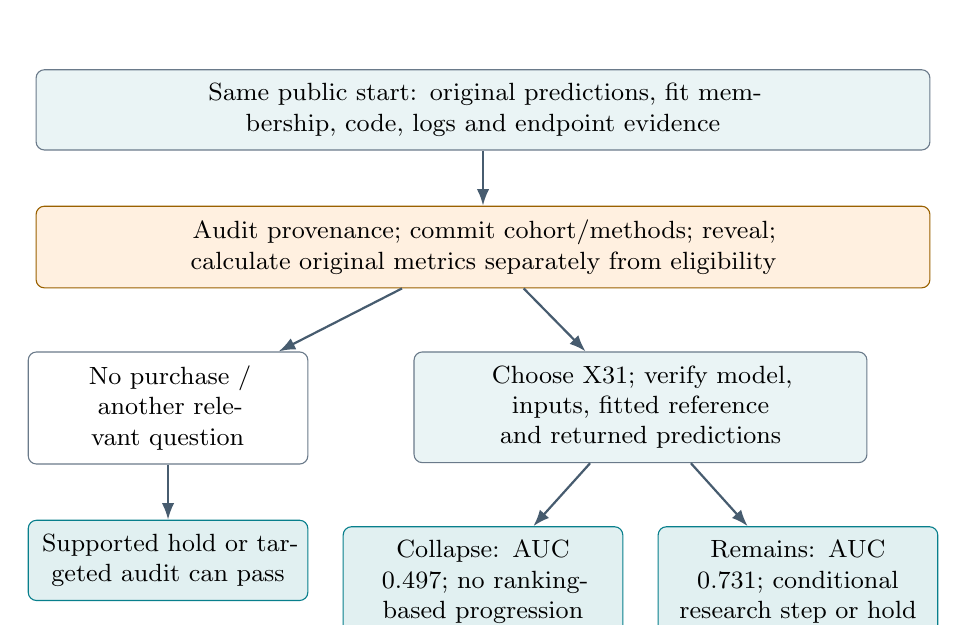
\begin{tikzpicture}[node distance=7mm]
\node[block,text width=11cm] (a) {Same public start: original predictions, fit membership, code, logs and endpoint evidence};
\node[gate,text width=11cm,below=of a] (b) {Audit provenance; commit cohort/methods; reveal; calculate original metrics separately from eligibility};
\node[neutral,text width=3.2cm,below=8mm of b.south,xshift=-4cm] (c) {No purchase / another relevant question};
\node[block,text width=5.4cm,below=8mm of b.south,xshift=2cm] (d) {Choose X31; verify model, inputs, fitted reference and returned predictions};
\node[result,text width=3.2cm,below=of c] (e) {Supported hold or targeted audit can pass};
\node[result,text width=3.2cm,below=8mm of d.south,xshift=-2cm] (f) {Collapse: AUC 0.497; no ranking-based progression};
\node[result,text width=3.2cm,below=8mm of d.south,xshift=2cm] (g) {Remains: AUC 0.731; conditional research step or hold};
\draw[arr] (a)--(b);\draw[arr] (b)--(c);\draw[arr] (b)--(d);
\draw[arr] (c)--(e);\draw[arr] (d)--(f);\draw[arr] (d)--(g);
\end{tikzpicture}
\caption{Case 3 evidence branches. Neither outcome retroactively authenticates the original export; retained ranking is not automatic probability-use approval.}
\end{figure}

\subsection{Reference calculations and causal limits}

\begin{table}[H]\small
\caption{Controlled reference results: group means, 100 group-bootstrap replicates, seed 19, 95\% interval, ten ECE bins. These are not model scores.}
\begin{tabularx}{\textwidth}{@{}Yrrrrr@{}}\toprule
Evidence & AUC & Interval & Brier & ECE & NB(0.5) \\\midrule
Original export & 1.00000 & [1.000,1.000] & 0.01487 & 0.11097 & 0.41071 \\
X31 collapse & 0.49736 & [0.414,0.615] & 0.29886 & 0.23148 & -0.02679 \\
X31 remains & 0.73057 & [0.622,0.821] & 0.20702 & 0.12186 & 0.08036 \\\bottomrule
\end{tabularx}
\end{table}

The retained condition passes the ranking gate, but its ECE of 0.12186 exceeds the existing 0.12 probability-use gate. A carefully scoped independent-validation step or an evidence-supported hold can both be defensible. Collapse cannot support progression based on ranking, but it also does not establish biological futility of anti-TNF prediction.

The modern paired inputs differ in patient--feature association, not just preprocessing fit scope. Consequently the pair is \emph{not} a controlled causal demonstration that removing leakage caused the observed AUC change. Validation membership in reference fitting also does not alone prove supervised outcome leakage. The report must keep fit provenance, evidence eligibility and biological explanation separate.

\subsection{Scoring, controls and work remaining}

Case 3 grades ten equally weighted properties: intended use/eligibility; cohort/dependence; fit provenance; prospective commitment; original calculations; containment of original invalidity; follow-up relevance; executable return when obtained; bounded decision; and reproducibility. Applicable weights are normalized; an unpurchased X31 return is N/A. Beliefs and scientific prose are diagnostic-only. A supported hold after a real investigation may pass both conditions, while generic answer-only policies fail.

Six reference workflows (two conditions times three estimands) pass at 100. The focused suite reports 102 passes; the then-current repository run reports 1,178 passes plus two already accepted historical RC1.4 provenance failures. Tests cover changed labels/predictions/fit membership, endpoint-window errors, copied paired results, unsupported claims, malformed inputs, method alternatives, Docker boundaries, provider exclusions and interrupted/restarted lifecycle states. These are recorded local controls, not external expert validation or new live-model evidence.

Remaining work is a bounded release audit, packaged production-path verification and separately approved calibration. The readiness report proposes Gemini on both conditions under \$10, followed by review; the complete three-model/two-condition design has a proposed \$40 cap. Its recorded no-cache base estimate is \$23.0247525 and its stress proxy is \$36.839604. Those are historical planning proxies based on earlier Case 2 tokens, not empirical median/P90 values or current prices. Refresh funding, route and token assumptions before authorization. No such execution is performed by this report.

\section{Case 4 roadmap: discrimination without usable probabilities}
\subsection{Existing task and evidence}

\textbf{Scientific question.} Does an attractive ranking score justify probability-threshold use, and is another experiment needed to decide that immediate question?

\textbf{Existing packet.} The historical case has 158 records representing 148 people across three sites, with two missing noncritical covariates. The sponsor claims AUC approximately 0.742 supports use at probability threshold 0.50. It supplies the same evidence categories and resource catalogue, with sealed validation labels and matched external returns.\cite{packet4,truth4}

\textbf{Required investigation for a future release.} Commit the biological unit and analysis; reconstruct AUC/uncertainty, Brier score, calibration, threshold confusion/net benefit and site sensitivity; distinguish ranking evidence from calibrated decision support; select new evidence only for a question that remains unresolved; restrict the final use.

\begin{figure}[H]\centering
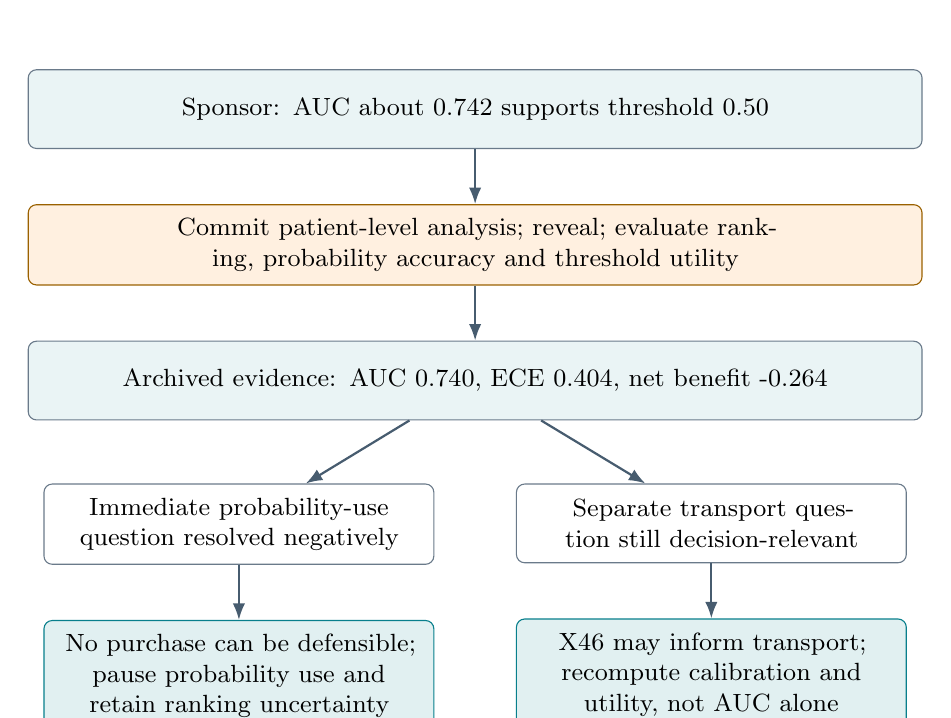
\begin{tikzpicture}[node distance=7mm]
\node[block,text width=11cm] (a) {Sponsor: AUC about 0.742 supports threshold 0.50};
\node[gate,text width=11cm,below=of a] (b) {Commit patient-level analysis; reveal; evaluate ranking, probability accuracy and threshold utility};
\node[block,text width=11cm,below=of b] (c) {Archived evidence: AUC 0.740, ECE 0.404, net benefit -0.264};
\node[neutral,text width=4.6cm,below=8mm of c.south,xshift=-3cm] (d) {Immediate probability-use question resolved negatively};
\node[neutral,text width=4.6cm,below=8mm of c.south,xshift=3cm] (e) {Separate transport question still decision-relevant};
\node[result,text width=4.6cm,below=of d] (f) {No purchase can be defensible; pause probability use and retain ranking uncertainty};
\node[result,text width=4.6cm,below=of e] (g) {X46 may inform transport; recompute calibration and utility, not AUC alone};
\draw[arr] (a)--(b);\draw[arr] (b)--(c);\draw[arr] (c)--(d);\draw[arr] (c)--(e);
\draw[arr] (d)--(f);\draw[arr] (e)--(g);
\end{tikzpicture}
\caption{Case 4 roadmap definition. The no-purchase branch reflects the agreed intended-use principle; the current legacy hidden whitelist has not yet been audited into a final release.}
\end{figure}

\subsection{Archived numerical reference}

\begin{table}[H]\small
\caption{Stored legacy Case 4 truth values. They were read for this report, not newly independently recomputed under a final MMMVP verifier.}
\begin{tabularx}{\textwidth}{@{}Yrr@{}}\toprule
Quantity & Original & Matched return \\\midrule
Patient AUC & 0.739713 & 0.796037 \\
Stored AUC interval & [0.651075,0.823517] & [0.682763,0.891168] \\
Brier & 0.331964 & 0.326544 \\
ECE & 0.403530 & 0.404928 \\
Net benefit at 0.50 & -0.263514 & -0.282609 \\
Naive row AUC & 0.742297 & Not tabulated \\
Site-weighted AUC & 0.717749 & Not tabulated \\
Worst-site AUC & 0.637500 & Not tabulated \\\bottomrule
\end{tabularx}
\end{table}

The archived numerical gates are AUC at least 0.70, interval lower bound at least 0.58, Brier at most 0.23, ECE at most 0.12 and net benefit at least zero. The stored pattern clears ranking gates but fails probability and utility gates. The fixed predictor need not be rebuilt to reach a valid negative decision about probability-based use. Recalibration and an independent evaluation of the recalibrated system would be a possible future investment, not a demonstrated remedy in this packet.

\subsection{Release work still required}

Case 4 has no current MMMVP audit, modern release closure, fresh calibrated model panel or accepted mission-score table. Historical v0.7/v0.8 work exists but is not promoted into present results. The old truth file explicitly lists X46 as the accepted/preferred purchase and pause/stop actions. Those legacy selectors cannot be presumed to implement the later rule that no purchase is acceptable when current evidence resolves the immediate probability-use question. This is an identified future audit issue, not an implemented repair.

The next work should inventory public disclosure and authoritative sources, independently recompute existing artifacts, test two valid workflows, verify no-purchase versus transport-question alternatives, and port proven optionality/lifecycle boundaries without importing case-specific verdicts. Numerical conventions, labels and fitted-processing provenance need review before any freeze. A further model call is premature until those local checks pass.

\section{Failure atlas and further experiments}

\begin{longtable}{@{}p{.20\textwidth}p{.28\textwidth}p{.27\textwidth}p{.17\textwidth}@{}}
\caption{Observed failure, capability hypothesis and resource that could address it. This is a research agenda, not measured intervention efficacy.}\\
\toprule Evidence & Observable behavior & Candidate resolving resource & What is established \\\midrule\endfirsthead
\toprule Evidence & Observable behavior & Candidate resolving resource & What is established \\\midrule\endhead
Case 1 Sonnet & Correct table exists, but decision-linked outputs cannot be replayed & Artifact-graph check or provenance tooling & Error and consequences observed; agent rescue untested. \\
Case 2 fresh Sonnet & Source-row counts equal entity counts incorrectly & Curator check of patient/visit mapping & Dependence-audit failure observed; intervention untested. \\
Case 2 historical Sonnet & Required cluster uncertainty absent & Statistical tool or biostatistician assistance & Missing requirement observed; reason for omission unknown. \\
Case 2 GPT-5.1 & Committed input is changed after reveal & Immutable-input tool/process & Prospective-integrity violation observed. \\
Case 2 X46 workflows & Relevant purchase is not turned into accepted decision evidence & Contingency design and evidence-binding support & Purchase alone did not complete the decision chain. \\
Cases 1--2 non-submitters & Useful intermediate work without accepted final artifact & Workflow memory, planning or interface assistance & Completion failure observed; budget versus interface contribution not isolated. \\
Case 3 paired references & Return may collapse or retain ranking & Executable evidence and subsequent independent validation & Reference outcomes known; agent recovery not measured. \\
Case 4 archived evidence & Attractive AUC with poor calibration and negative utility & Calibration review plus independent validation of any changed predictor & Legacy numerical pattern only; no tested remedy. \\\ottomrule
\end{longtable}

Every future intervention comparison should predeclare the failure property, supplied resource and paired control, hold task science constant, and measure recovery in both direct quality and mission completion. Additional data, metadata, expert help, process tools and model adaptation are competing possibilities. SFT, RL, retrieval or prompting should only be claimed effective when the corresponding intervention is tested.

Repeated attempts should report always/sometimes/never successful behavior with denominators, cost and uncertainty. The two Case 3 conditions share a common case and must not be treated as independent biological studies. Breaking-point curves require predeclared perturbation ladders and repeated observations; none is plotted as an empirical result here. In future, both cumulative failure and later containment/recovery should be shown, so a single early fault does not hide useful downstream work.

\section{Packaging, limitations and handoff}

\subsection{Current Case 2 package evidence}

The inspected \texttt{uc-bench-case2-mmmvp-v1} candidate contains 25 agent-visible files, 406 host-only files and 1,287 evidence files. Two clean builds produce identical public and host archives. Replay parity passes on all four preserved trajectories; the active-code audit reports no unexplained history-specific scoring hits. The public-file scan reports no credential-shaped strings or exact hidden-file content hits. These are records of specific tests, not a universal security proof.\cite{c2package}

The manifest's status is \texttt{candidate\_unfrozen}. Its aggregate candidate digest is listed in Appendix~\ref{sec:manifest}. No final Case 2 release-freeze artifact was present in the inspected top-level package evidence. A later signed-off freeze can update the status page without rewriting historical trajectory outcomes. The main task's ongoing work is outside this report's execution scope.

\subsection{Principal validity limitations}

\begin{enumerate}
\item \textbf{Small, exposed development sample.} Case 1 has four eligible attempts and one provider exclusion; Case 2 has four attempts across three models. Repairs used exposed trajectories plus general controls. There is no untouched final evaluation here.
\item \textbf{Controlled data.} The packet results are controlled diligence exercises, not demonstrated clinical or authentic-cohort performance. Public literature contamination and controlled template recognition remain distinct risks.
\item \textbf{Interface burden.} Disclosed schemas avoid hidden traps but still consume work. Rejected plans, source-link bookkeeping and turn-limit failures need separate empirical measurement before calling all losses scientific.
\item \textbf{Limited semantic interpretation.} Strict graders rely on disclosed machine fields and saved artifacts. Unexpressed reliance on an optional uncertainty sub-result cannot be inferred from prose in the current Case 2 contract.
\item \textbf{Residual reporting differences.} Case 1 excludes unsubmitted science scores; Case 2 retains partial work. A Case 2 strict/diagnostic artifact-graph distinction and Case 1 turn-counter differences are disclosed rather than harmonized after the fact.
\item \textbf{No external expert validation.} Internally authored references and independent implementations test engineering consistency but do not replace clinical/statistical specialist validation.
\item \textbf{Reward signal not yet training efficacy.} Partial scores may be useful RL signals, but optimizing them could emphasize artifact production. Training utility and resistance to strategic reward optimization have not been demonstrated by this pilot.
\end{enumerate}

\subsection{Further work in order}

\begin{enumerate}
\item Complete and record the Case 2 packaging/freeze decision, retaining the two validated general corrections and the current evidence provenance.
\item Perform Case 3's bounded release audit using existing datasets and both current controlled returns; refresh local execution and cost assumptions before any live tranche.
\item Audit Case 4's legacy task/claim/resource semantics and independently recompute the existing data before proposing implementation changes.
\item Only after release readiness, predeclare a small balanced repeated-attempt design with explicit completion, scientific and infrastructure denominators.
\item Run targeted paired interventions to distinguish data, metadata, expertise, tools and model-adaptation hypotheses. Keep observed behavior separate from hypothesized training causes.
\end{enumerate}

\appendix
\section{Release digests and evidence index}\label{sec:manifest}

\small
\begin{longtable}{@{}p{.30\textwidth}p{.63\textwidth}@{}}
\toprule Artifact & Recorded SHA-256 / status \\\midrule\endfirsthead
\toprule Artifact & Recorded SHA-256 / status \\\midrule\endhead
Case 1 RC6 release & \filepath{a1795f1be20b02bb02d86516a664a3d62aed7d6ca716bdd45cb277b4c1ea6d19} \\
Case 2 frozen budget1 & \filepath{3233cff94612fa75d80ebbe80468df5a4c73a0ead64d8d7327c01825d3436b4c} \\
Case 2 MMMVP candidate & \filepath{0ca0d1c1ce661a387d94747767594fc3c3ad6820a99c535cf2c8d37d1a6a222e}; candidate\_unfrozen \\
Case 2 public archive & \filepath{3c363ff0b71842c8b2eaddaac4c2102a0f1688ee87f2c25a6ea18e0c871e85b6} \\
Case 2 host archive & \filepath{0989e08d4f5247c6816475924a954b8d893cfffb6eb9e7d587ce4b493dec9e14} \\
Case 3 development closure & \filepath{2083d5fd4380b3da933dc78e39bbcadb883eb18ce9bda66e4c3247a3ad5ab9ae}; unfrozen candidate \\
Case 3 identical public start & \filepath{2515f2963cb06cdda331ff1159ae9b8cc75daa37398b0412391f65a001bd180a} \\
Case 4 & No current MMMVP release digest established in this report. \\\bottomrule
\end{longtable}
\normalsize

\section{Reproduction and document compilation}

\textbf{Overleaf.} Create a blank project; upload this file as \texttt{main.tex}; select pdfLaTeX and compile. Diagrams use TikZ/PGFPlots; references are embedded. No external images, shell escape, datasets, API key or bibliography file are required. Recompile to resolve the contents and cross-references.

\textbf{Repository evidence.} All repository-relative paths in the references are under the UC-Bench project root. This report is an analysis artifact and does not mutate releases, execute models or authorize new spend. The listed commands are documented entry points, not a claim that they were run while preparing this report:
\begin{lstlisting}
# Case 2 packaged fake-provider lifecycle (requires local project setup + Docker)
PYTHONPATH=src:. .venv.nosync/bin/python scripts/run_case2_mmmvp_v1.py --fake

# Case 2 preserved trajectory replay through the packaged verifier
PYTHONPATH=src:. .venv.nosync/bin/python scripts/replay_case2_mmmvp_v1.py
\end{lstlisting}

\textbf{Source hierarchy.} Prefer accepted release reports and machine replay artifacts to earlier design cards. In particular, the old Case 3 card's ``opposite decisions required'' and ``leakage caused the score'' language is superseded by the current locally validated provenance specification. Case 4 remains legacy material with unresolved release semantics. Unsupported values are marked missing; no new model runs or numerical ground-truth recomputations were performed for this document.

\begin{thebibliography}{99}\small
\bibitem{c1} UC-Bench. \emph{Case 1 RC6 final report}. \filepath{reports/uc_bench_case1_pilot_v1_rc6_final.md}. Associated \filepath{artifacts/uc_bench_case1_pilot_v1_rc6/science/pilot_report.json}, RC5/RC6 run summaries and saved primary outputs.
\bibitem{runbook} UC-Bench. \emph{Case 2 MMMVP v1 runbook and score sources}. \filepath{docs/CASE2_MMMVP_V1_RUNBOOK.md}; \filepath{docs/CASE2_MMMVP_V1_SCORE_SOURCES.md}.
\bibitem{c2run} UC-Bench. \emph{Case 2 graceful-failure calibration results}. \filepath{reports/UC_BENCH_CASE2_GRACEFUL_CALIBRATION_RESULTS.md}; preserved summaries under \filepath{artifacts/uc_bench_case2_graceful_budget_calibration/science/runs/}.
\bibitem{c2diag} UC-Bench. \emph{Case 2 diagnostic-scoring repair}. \filepath{reports/UC_BENCH_CASE2_DIAGNOSTIC_SCORING_REPAIR.md}.
\bibitem{c2canary} UC-Bench. \emph{Case 2 fresh diagnostic canary}. \filepath{reports/UC_BENCH_CASE2_DIAGNOSTIC_CANARY.md}; preserved canary run summary and adjudication.
\bibitem{c2optional} UC-Bench. \emph{Case 2 strict-verifier optionality repair}. \filepath{reports/UC_BENCH_CASE2_OPTIONALITY_REPAIR.md}; \filepath{artifacts/uc_bench_case2_optionality_repair/replays.json}; \filepath{development/case2_optionality_repair/SINGLE_AUTHORITY_TABLE.md}.
\bibitem{c2package} UC-Bench. \emph{Case 2 MMMVP package candidate evidence}. \filepath{artifacts/uc_bench_case2_mmmvp_v1/candidate_manifest.json}, \filepath{build_reproducibility.json}, \filepath{replay_parity.json}, and \filepath{anti_overfitting_audit.json} in that directory.
\bibitem{c3} UC-Bench. \emph{Case 3 MMMVP local readiness and implementation specification}. \filepath{reports/UC_BENCH_CASE3_MMMVP_LOCAL_READINESS.md}; \filepath{reports/CASE3_MMMVP_IMPLEMENTATION_SPEC.md}; \filepath{artifacts/uc_bench_case3_mmmvp/local_validation_01/}.
\bibitem{c4status} UC-Bench. \emph{Four-case MMMVP status}, 13 September 2026. \filepath{reports/UC_BENCH_FOUR_CASE_EOD_STATUS.md}. Used for Case 4 status only; its earlier Case 2 status is superseded.
\bibitem{packet4} UC-Bench. \emph{Case 4 historical public packet}. \filepath{tasks/hard_suite_v07/development/case_04/}: intended use, README, sponsor assertions and follow-up catalogue.
\bibitem{truth4} UC-Bench. \emph{Case 4 historical reference truth}. \filepath{grader_private/hard_suite_v07/case_04/truth.json}. Stored values, not a current independent verification.
\end{thebibliography}
\end{document}
